%!TEX root = paper.tex

\section{Browsers}
\label{sec:browsers}

Modern web browsers do not just load static pages, but can also handle pages that have similar
complexity to native applications.
From application suites such as the Google Apps\footnote{\url{https://apps.google.com}} to games
based on the Unreal Engine\footnote{\url{https://www.unrealengine.com/}},
modern browsers have the ability to handle much more than simple static pages.
\figref{fig:browser} shows the steps in processing a site.
While the naming is specific to the Servo browser, similar steps are used in all modern browsers.\footnote{\url{http://www.html5rocks.com/en/tutorials/internals/howbrowserswork/}}
\begin{figure*}[ht]
  \begin{center}
    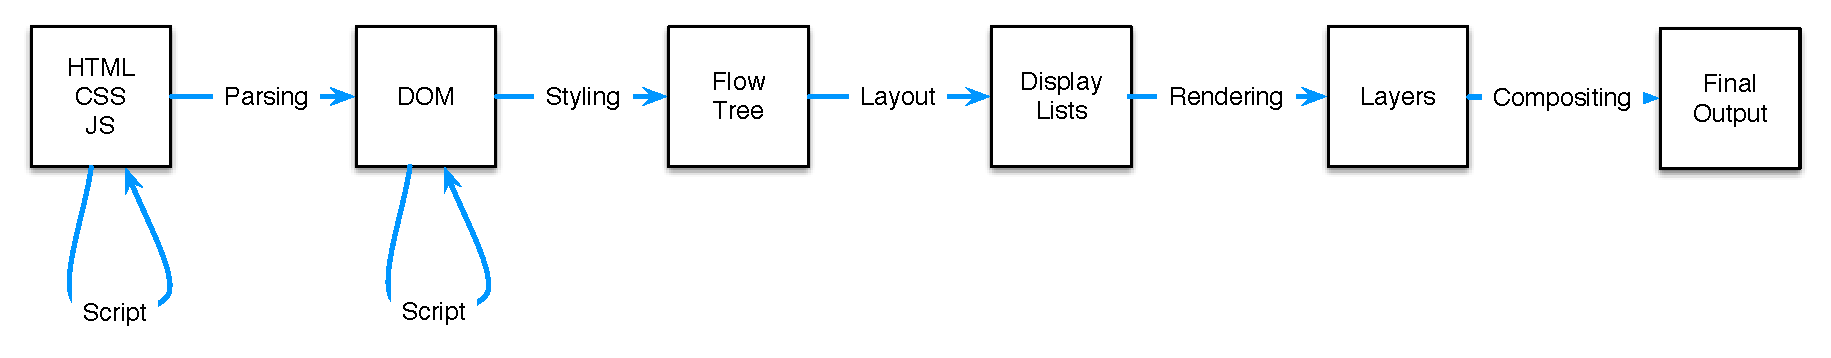
\includegraphics[scale=0.7]{pics/browser}
  \end{center}%
  \caption{Processing stages and intermediate representations in a browser engine.}
  \label{fig:browser}
\end{figure*}%

\subsection{Parsing HTML and CSS}

A URL identifies a resource to load.
This resource usually consists of HTML, which is then parsed and typically turned into a Document Object
Model (DOM) tree.
From a programming languages standpoint, there are several interesting aspects of the parser design
for HTML.
First, though the specification allows the browser to abort on a parse error\footnote{\url{https://html.spec.whatwg.org/multipage/#parsing}},
in practice browsers follow the recovery algorithms described in that specification precisely so that
even ill-formed HTML will be handled in an interoperable way across all browsers.
Second, due to the presence of the \lstinline[language=HTML]{<script>} tag, the token stream can be modified
during operation.
For example, the below example that injects an open tag for the header and comment blocks works in all modern browsers.
\begin{lstlisting}[language=HTML]
<html>
  <script>
  document.write("<h")\';
  </script>1>
  This is a h1 title

  <script>
  document.write("<!-");
  </script>-
  This is commented
  -->
</html>
\end{lstlisting}
This requires parsing to pause until JavaScript code has run to completion.
But, since resource loading is such a large factor in the latency of loading many webpages (particularly on mobile),
all modern parsers also perform speculative token stream scanning and prefetch of resources likely to be required~\cite{browsers-slow-smartphones}.

\subsection{Layout}

After constructing the DOM and determining the set of styles defined in the Cascading Style Sheets (CSS) that has
been loaded, those styles are applied to the DOM and a new flow tree that represents the elements is created.
This process can create many more flows than previously existed in the DOM --- for example, when a list item is
styled to have an associated counter glyph.

\subsection{Display}

That tree of elements, called the \emph{flow tree} in Servo, is then processed
to produce a set of \emph{display list} items.  These list items are the
actual graphical elements, text runs, etc. in their final on-screen positions.
The order in which these elements are displayed is well-defined by the
standard\footnote{\url{http://www.w3.org/TR/CSS21/zindex.html#painting-order}}.

\subsection{Rendering}

Once all of the elements to appear on screen have been computed, these
elements are rendered, or painted, into memory buffers or directly to graphics
surfaces.

\subsection{Compositing}

The set of memory buffers or graphical surfaces, called layers, are then
transformed and composited together to form a final image for
presentation.

\subsection{Scripting}

Whether through timers, \lstinline[language=HTML]{<script>} blocks in the
HTML, user interactions, or other event handlers, JavaScript code may execute
at any point during parsing, layout, and painting or afterwards during
display.  These scripts can modify the DOM tree, which may require rerunning
the layout and painting passes in order to update the output.  Most modern
browsers use some form of dirty bit marking to attempt to minimize the
recalculations during this process.


%%% Local Variables: 
%%% mode: latex
%%% TeX-master: "paper"
%%% End: 
